\documentclass[border=10pt]{standalone}

\usepackage{tikz}
\usepackage{tikzsymbols}
\usetikzlibrary{calc,patterns,shapes.geometric}

\def\centerarc[#1](#2)(#3:#4:#5){\draw[#1] ($(#2)+({#5*cos(#3)},{#5*sin(#3)})$) arc (#3:#4:#5);}

\begin{document}
	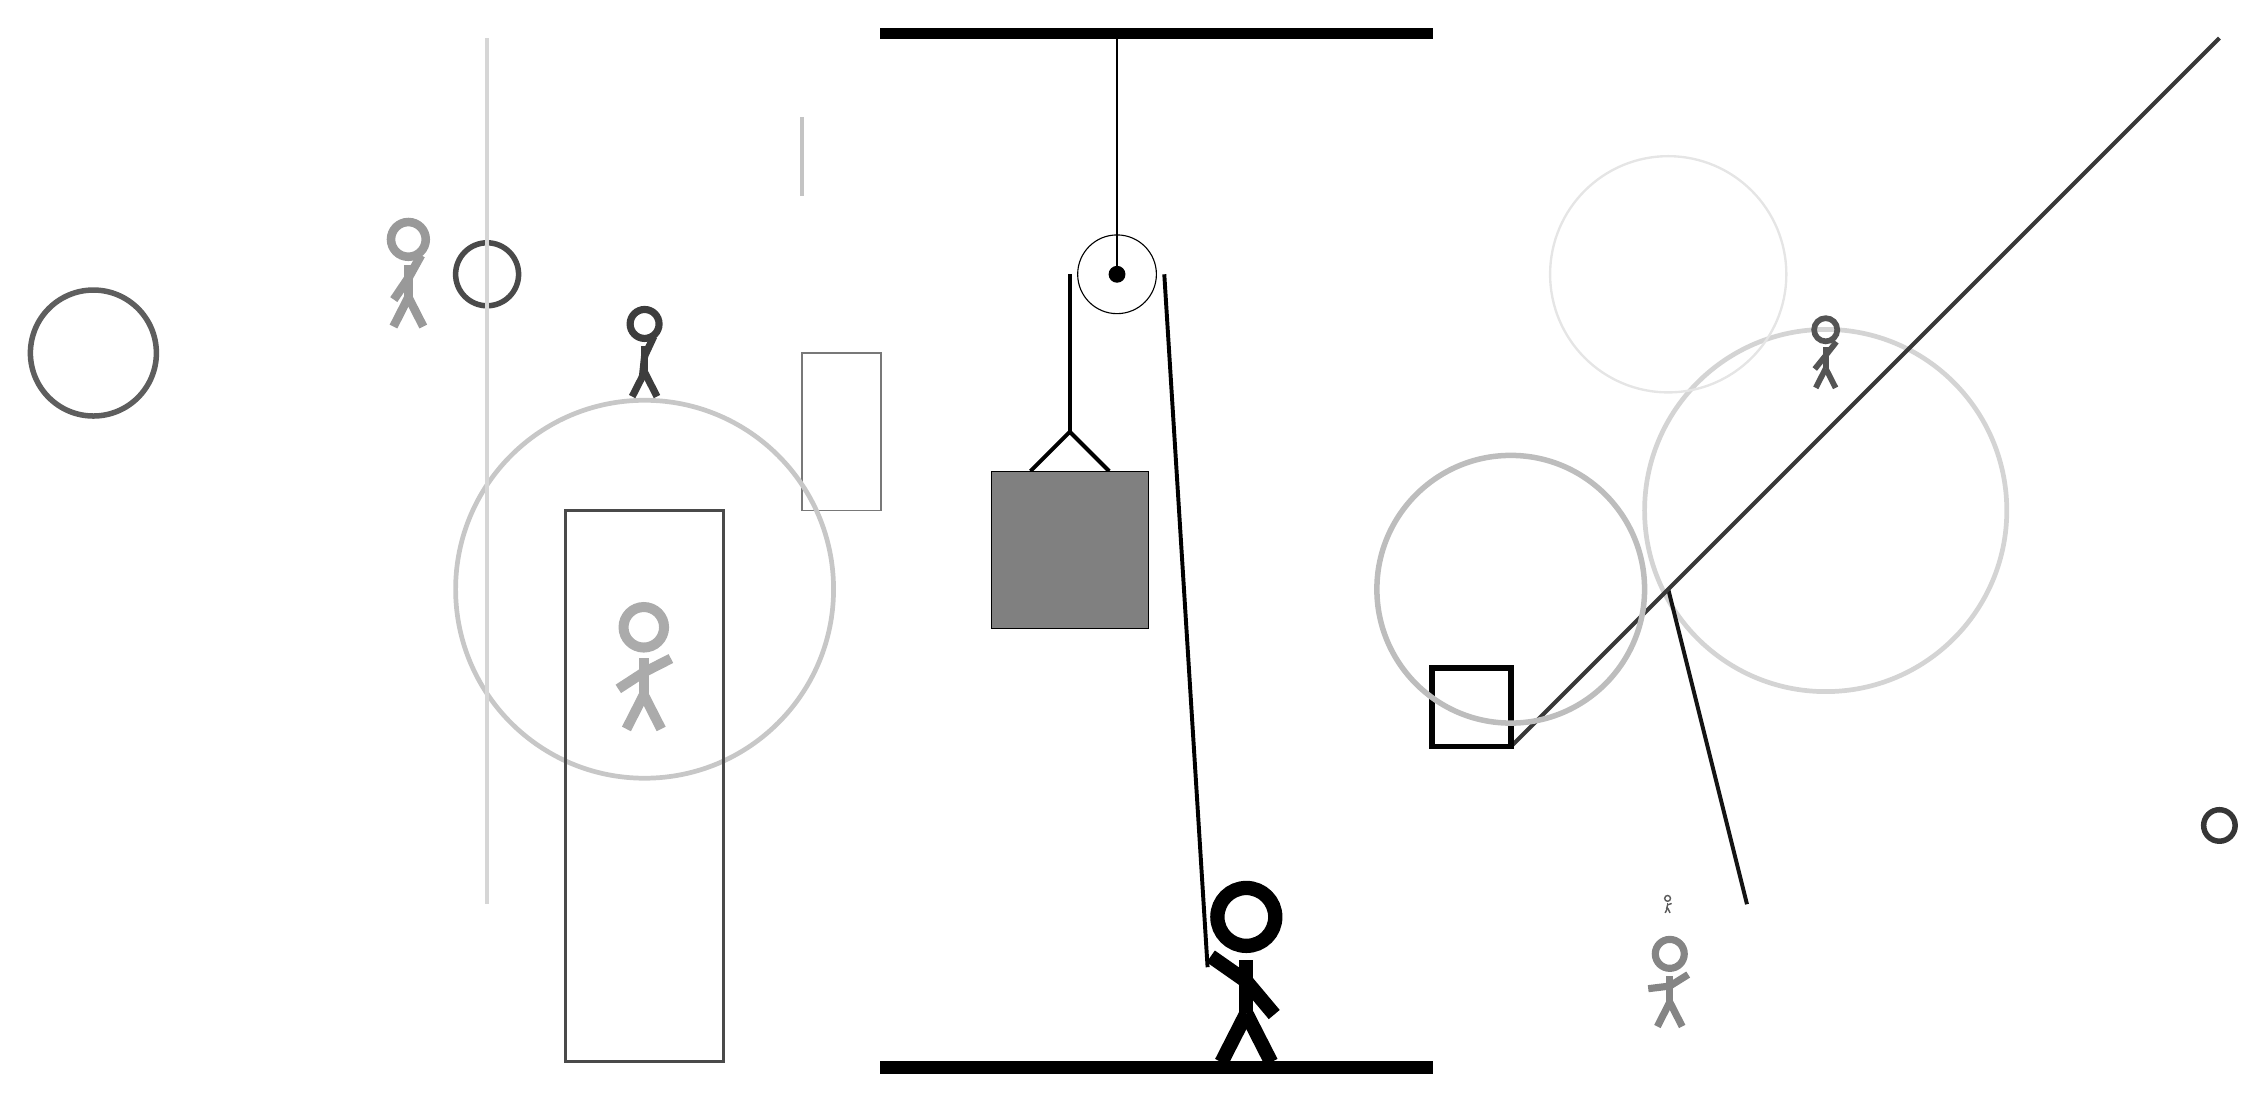
\begin{tikzpicture}
		%%%%% START %%%%%
		
		\draw[fill=black] (-2, 10) rectangle (5, 10.125);
		
		\draw (1, 7) circle (0.5);
		\draw[fill=black] (1, 7) circle (0.1);
		\draw (1, 10) -- (1, 7);
		
		\draw[line width=0.5mm] (-0.1, 4.5) -- (0.4, 5.0) -- (0.9, 4.5);
		\draw[fill=black!50] (-0.6, 4.5) rectangle (1.4, 2.5);
		
		\draw[line width=0.5mm] (0.4, 7) -- (0.4, 5.0);
		\centerarc[line width=0.5mm](1, 7)(0:180:0.6);
		\draw[line width=0.5mm](1.6, 7) -- (2.15, -1.8);
		
		\node[line width=0.4mm, color=black!33] at (-5, 2) {\Strichmaxerl[7][33][27]};
		
		\draw [line width=0.6mm, color=black!17](10, 4) circle (2.3);
		\draw [line width=0.7mm, color=black!63](-12, 6) circle (0.8);
		\draw[line width=0.5mm, color=black!92](8, 3) -- (9, -1);
		\draw[line width=0.2mm, color=black!53] (-2, 4) rectangle (-3, 6);
		\draw [line width=0.6mm, color=black!22](-5, 3) circle (2.4);
		\draw[line width=0.5mm, color=black!78](6, 1) -- (15, 10);
		
		\draw[line width=0.7mm, color=black!99] (5, 2) rectangle (6, 1);
		\node[line width=0.6mm, color=black!40] at (-8, 7) {\Strichmaxerl[6][56][61]};
		\node[line width=0.2mm, color=black!48] at (8, -2) {\Strichmaxerl[5][7][32]};
		\draw [line width=0.7mm, color=black!71](-7, 7) circle (0.4);
		\draw[line width=0.4mm, color=black!71] (-4, 4) rectangle (-6, -3);
		\draw[line width=0.5mm, color=black!16](-7, 10) -- (-7, -1);
		
		\node[line width=0.5mm, color=black!64] at (8, -1) {\Strichmaxerl[1][76][18]};
		\draw [line width=0.7mm, color=black!26](6, 3) circle (1.7);
		\draw[line width=0.5mm, color=black!23](-3, 9) -- (-3, 8);
		\node[line width=0.5mm, color=black!67] at (10, 6) {\Strichmaxerl[4][51][52]};
		
		\node[line width=0.5mm, color=black!76] at (-5, 6) {\Strichmaxerl[5][84][65]};
		\draw [line width=0.3mm, color=black!10](8, 7) circle (1.5);
		
		\draw [line width=0.7mm, color=black!79](15, 0) circle (0.2);
		
		\node at (2.6, -1.9) {\Strichmaxerl[10][-35][-50]};
		
		\draw[fill=black] (-2, -3) rectangle (5, -3.15);
		
		%%%%% END %%%%%
	\end{tikzpicture}
\end{document}